%%%%%%%%%%%%%%%%%%%%%%%%%%%%%%%%%%%%%%%%%
%
% (c) 2020 by Jennifer Laaser
%
% This work is licensed under the Creative Commons Attribution-NonCommercial-ShareAlike 4.0 International License. To view a copy of this license, visit http://creativecommons.org/licenses/by-nc-sa/4.0/ or send a letter to Creative Commons, PO Box 1866, Mountain View, CA 94042, USA.
%
% The current source for these materials is accessible on Github: https://github.com/jlaaser/pogil-polymers
%
%%%%%%%%%%%%%%%%%%%%%%%%%%%%%%%%%%%%%%%%%

\documentclass[instructor,handout]{pogil}
%\documentclass[handout]{pogil}

%%%%%%%%%%%%%%%%% DOCUMENT INFORMATION %%%%%%%%%%%%%%%%%%%%%%%%

\copyrightshort{
\includegraphics[width=0.1\textwidth]{by-nc-sa} J. Laaser 2020}

%%%%%%%%%%%%%%%%%%%%%%%%%%%%%%%%%%%%%%%%%%%%%%%%%%%%%%%%%%%%%%%%%
%%%%%%%%%%%%%%%%%%%%%%%%%%%%%%%%%%%%%%%%%%%%%%%%%%%%%%%%%%%%%%%%%

\begin{document}
	
% to change the activity output in the pdf, change this to the file path for the activity you want to include:
%%%%%%%%%%%%%%%%%%%%%%%%%%%%%%%%%%%%%%%%%%
%
% (c) 2018 by Jennifer Laaser
%
% This work is licensed under the Creative Commons Attribution-NonCommercial-ShareAlike 4.0 International License. To view a copy of this license, visit http://creativecommons.org/licenses/by-nc-sa/4.0/ or send a letter to Creative Commons, PO Box 1866, Mountain View, CA 94042, USA.
%
% The current source for these materials is accessible on Github: https://github.com/jlaaser/pogil-polymers
%
%%%%%%%%%%%%%%%%%%%%%%%%%%%%%%%%%%%%%%%%%

\section{Activity Template}
\renewcommand{\figpath}{content/figs}

\textbf{Focus question:} Put a central question for the students to consider through this exercise here.

\subsection{Model 1:  ABC}

Here is the first model for students to consider

% to include images, put them in the folder specified by figpath and then use:
%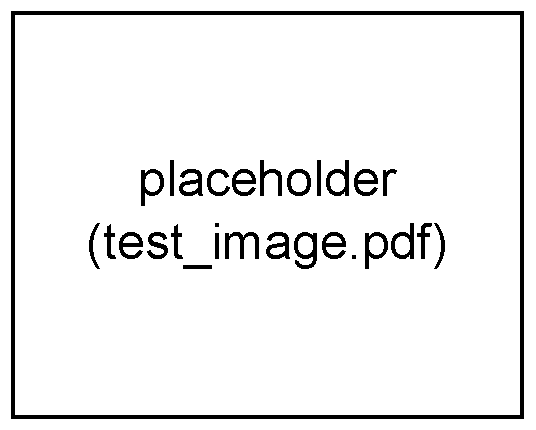
\includegraphics[width=0.8\textwidth]{\figpath/test_image.pdf}

\subsection{Critical Thinking Questions}

	\begin{enumerate}
		\item First question?
		\item Second question?
	\end{enumerate}

\subsection{Model 2: DEF}

\subsection{Critical Thinking Questions}

	\begin{enumerate}
		\item First question?
		\item Second question?
	\end{enumerate}

\subsection{Exercises}

	After class, \textbf{read} the following sections of your textbook:
	
	\begin{enumerate}
		\item First section
		\item Second section
	\end{enumerate}
	
	Then, do the following exercises:
	
	\begin{enumerate}
		\item First exercise
		\item Second exercise
	\end{enumerate}
%%%%%%%%%%%%%%%%%%%%%%%%%%%%%%%%%%%%%%%%%
%
% (c) 2019 by Jennifer Laaser
%
% This work is licensed under the Creative Commons Attribution-NonCommercial-ShareAlike 4.0 International License. To view a copy of this license, visit http://creativecommons.org/licenses/by-nc-sa/4.0/ or send a letter to Creative Commons, PO Box 1866, Mountain View, CA 94042, USA.
%
% The current source for these materials is accessible on Github: https://github.com/jlaaser/pogil-polymers
%
%%%%%%%%%%%%%%%%%%%%%%%%%%%%%%%%%%%%%%%%%

\renewcommand{\figpath}{content}
\renewcommand{\labelbase}{FRPkinetics}

\begin{activity}[Kinetics of Free-Radical Polymerization]

\begin{instructornotes}
	This activity introduces students to concepts related to the kinetics of free-radical polymerization.
	
	After completing this activity, students will be able to:
	\begin{enumerate}
		\item Write kinetic equations for each of the major steps of a free-radical polymerization
		\item Calculate the kinetic chain length for a free-radical polymerization
	\end{enumerate}
	
	\subsection*{Activity summary:}
	\begin{itemize}
		\item \textbf{Activity type:} Learning Cycle
		\item \textbf{Content goals:} Kinetics of free-radical polymerization
		\item \textbf{Process goals:} %https://pogil.org/uploads/attachments/cj54b5yts006cklx4hh758htf-process-skills-official-pogil-list-2015-original.pdf
			written communication, critical thinking, information processing
		\item \textbf{Duration:} TBD
		\item \textbf{Instructor preparation required:} none beyond knowledge of relevant content
		\item \textbf{Related textbook chapters:}
			\begin{itemize}
				\item \emph{Polymer Chemistry} (Hiemenz \& Lodge): section NNN
			\end{itemize}
		%\item \textbf{Facilitation notes:}
		%	\begin{itemize}
		%		\item \dots
		%	\end{itemize}
	\end{itemize}
	
\end{instructornotes}


\begin{model}[Kinetic Equations]
	\label{\labelbase:mdl:kineticeqns}

	Rate laws for some common types of chemical reactions are shown below:
	
	\vspace{-6pt}
	\begin{center}
		\renewcommand{\arraystretch}{2}
		\begin{tabular}{c c c c}
			\hspace{2cm}\textbf{Reaction:}\hspace{2cm} & \multicolumn{3}{c}{\hspace{0.5cm}\textbf{Rate laws:}\hspace{0.5cm}} \\
			$ \text{A} \xlongrightarrow{k} \text{B}$ & $\frac{d[\text{A}]}{dt} = -k[\text{A}]$ && $\frac{d[\text{B}]}{dt} = k[\text{A}]$ \\
			$ \text{A} \xlongrightarrow{k} 2\text{ B}$ & $\frac{d[\text{A}]}{dt} = -k[\text{A}]$ && $\frac{d[\text{B}]}{dt} = 2k[\text{A}]$ \\
			$\text{2 A} \xlongrightarrow{k} \text{B}$ & $\frac{d[\text{A}]}{dt} = -2k[\text{A}]^2$ && $\frac{d[\text{B}]}{dt} = k[\text{A}]^2$ \\
			$\text{A + B} \xlongrightarrow{k} \text{C}$ & $\frac{d[\text{A}]}{dt} = -k[\text{A}][\text{B}]$ && $\frac{d[\text{C}]}{dt} = k[\text{A}][\text{B}]$ \\
			$\text{A + B} \xlongrightarrow{k} \text{2 C}$ & $\frac{d[\text{A}]}{dt} = -k[\text{A}][\text{B}]$ && $\frac{d[\text{C}]}{dt} = 2 k[\text{A}][\text{B}]$ \\
			$\text{A + B} \xlongrightarrow{k} \text{C + D}$ & $\frac{d[\text{A}]}{dt} = -k[\text{A}][\text{B}]$ && $\frac{d[\text{C}]}{dt} = k[\text{A}][\text{B}]$ \\
		\end{tabular}
	\end{center}
	\vspace{6pt}
	
\end{model}


\begin{ctqs}

	\question The first step in a free-radical polymerization is \emph{initiation}.  
		
		\begin{enumerate}
		
			\item First, an initiator molecule decomposes to create initiator radicals:
				\begin{equation*}
					\text{Init} \xlongrightarrow{k_d} \text{2 \ce{I^.}}
				\end{equation*}	
				Write an expression for the rate at which new initiator radicals are generated, $\frac{d[\text{I}^{\bullet}]}{dt}$, in terms of the concentration of initiator, [Init], and dissociation constant, $k_d$.
		
				\begin{solution}[1.25in]
				\end{solution}
		
			\item If a fraction $f$ of the initiator radicals successfully go on to generate new polymer chain radicals (\ce{P^.}), what is the overall initiation rate of polymer chains, $\frac{d[\text{\ce{P^.}}]}{dt}$?
		
				\begin{solution}[1.25in]
				\end{solution}
		
		\end{enumerate}
		
	\question The second step in a free-radical polymerization is propagation:
		\begin{equation*}
			\text{\ce{P_i^.} + M} \xlongrightarrow{k_p} \text{\ce{P_{i+1}^.}}
		\end{equation*}
		
		Generally, we make the approximation that all of the polymer radicals are equally reactive and are ``equivalent'' to each other regardless of chain length, so we summarize this reaction as
		\begin{equation*}
			\text{\ce{P^.} + M} \xlongrightarrow{k_p} \text{\ce{P^.}}
		\end{equation*}
		where [\ce{P^.}] is the \emph{total} concentration of propagating radical chains.
	
		Write an expression for $-\frac{d[\text{M}]}{dt}$, the rate at which monomers are used up, in terms of the radical concentration, [\ce{P^.}], the monomer concentration, [M], and the propagation rate constant, $k_p$.
		
		\begin{solution}[1.25in]
		\end{solution}
		
	\question The final step in a free-radical polymerization is termination:
		\begin{align*}
			\text{\ce{P^.} + \ce{P^.}} \xlongrightarrow{k_{t,c}} \text{\ce{PP}} && \text{or} && \text{\ce{P^.} + \ce{P^.}} \xlongrightarrow{k_{t,d}} \text{P + P}\\
			\text{combination\hspace{0.5cm}} && && \text{disproportionation}
		\end{align*}
		
		\begin{enumerate}
			\item For termination by combination, write an expression for $-\frac{d[\text{P}^{\bullet}]}{dt}$ in terms of the radical concentration, [\ce{P^.}], and the rate constant, $k_{t,c}$.
			
				\begin{solution}[0.75in]
				\end{solution}
			
			\item For termination by disproportionation, write an expression for $-\frac{d[\text{P}^{\bullet}]}{dt}$ in terms of the radical concentration, [\ce{P^.}], and the rate constant, $k_{t,d}$.
			
				\begin{solution}[0.75in]
				\end{solution}
			
			\item Combine your answers to the previous two questions to find an expression for the \emph{total} rate at which propagating radicals are removed from the reaction, in terms of the radical concentration, [\ce{P^.}], and the total termination rate constant, $k_t = k_{t,c} + k_{t,d}$.
			
				\begin{solution}[0.75in]
				\end{solution}
				
		\end{enumerate}

\end{ctqs}



\begin{model}[Summary of Free-Radical Kinetics]
\label{\labelbase:mdl:kineticssummary}

	The major reaction steps in free-radical polymerization and their rate laws are summarized below:
	
	\begin{center}
		\renewcommand{\arraystretch}{2}
		\begin{tabular}{c c c}
			\textbf{Step:} & \textbf{Overall Reaction:} & \textbf{Rate:}\\\hline
			\multirow{2}{*}{Initiation} & $[\text{Init}] \xlongrightarrow{k_d} \text{2 \ce{I^.}}$ & \multirow{2}{*}{$ R_i = \frac{d\text{[\ce{P^.}]}}{dt} = 2fk_d[\text{Init}]$}\\
			 & $\text{\ce{I^.} + M} \xlongrightarrow{k_i} \text{\ce{P^.}}$ & \\\hline
			Propagation & $\text{\ce{P^.} + M} \xlongrightarrow{k_p} \text{\ce{P^.}}$ & $R_p = -\frac{d[\text{M}]}{dt} = k_p\text{[M][\ce{P^.}]}$\\\hline
			\multirow{2}{*}{Termination} & $\text{\ce{P^.} + \ce{P^.}} \xlongrightarrow{k_{t,c}} \text{\ce{PP}}$ & \multirow{2}{*}{$R_t = -\frac{d[\text{\ce{P^.}}]}{dt} = 2k_t [\text{\ce{P^.}}]^2$}\\
			& $\text{\ce{P^.} + \ce{P^.}} \xlongrightarrow{k_{t,d}} \text{P + P}$ & \\\hline
		\end{tabular}
	\end{center}
	\vspace{6pt}

\end{model}

\begin{ctqs}

	\question Which rate ($R_i$, $R_p$, or $R_t$) describes...
	
		\begin{enumerate}
			\item ... the rate at which new propagating polymer radicals are generated?
			
				\begin{solution}[0.5in]
				\end{solution}
				
			\item ... the rate at which monomers are incorporated into polymer?
			
				\begin{solution}[0.5in]
				\end{solution}
				
			\item ... the rate at which propagating polymer radicals are removed from the reaction?
			
				\begin{solution}[0.5in]
				\end{solution}
				
		\end{enumerate}

	\question To simplify the kinetic equations shown in Model \ref{\labelbase:mdl:kineticssummary}, we assume that the concentration of radicals reaches a ``steady state'', where [\ce{P^.}] is constant.
	
		\begin{enumerate}
			\item One way to ensure that $[\text{P}^{\bullet}]$ reaches a steady state is to require that the rate at which polymer radicals are \emph{generated} is equal to the rate at which they are \emph{removed} from the reaction.
			
				Which two rates ($R_i$, $R_p$, and/or $R_t$) must be equal for this to be true?
				
				\begin{solution}[0.75in]
				\end{solution}
				
			\item Set the two rates identified in the previous question equal to each other and solve for $[\text{P}^{\bullet}]$ in terms of $f$, $k_d$, $k_t$, and $[\text{Init}]$.
			
				\begin{solution}[2in]
					\begin{align*}
						R_i &= R_t \\
						2fk_d[Init] &= 2k_t[P^\bullet]^2\\
						[P^\bullet]^2 &= \frac{fk_d[Init]}{k_t}\\
						[P^\bullet] &= \left(\frac{fk_d[Init]}{k_t}\right)^{1/2}
					\end{align*}
				\end{solution}
			
			\item Finally, use your answer to find an expression for the polymerization rate, $R_p$, in terms of $f$, $k_d$, $k_p$, $k_t$, $[\text{M}]$, and $[\text{Init}]$.
			
				\begin{solution}[1.5in]
					\begin{align*}
						R_p &= k_p\text{[M][\ce{P^.}]}\\
						&= k_p\text{[M]}\left(\frac{fk_d[Init]}{k_t}\right)^{1/2}
					\end{align*}
				\end{solution}
			
		\end{enumerate}
	
	\question Consider a period of time, $\Delta t$, at the start of the reaction.
	
		\begin{enumerate}
			
			\item How many monomers do you expect to be incorporated into polymer chains in this time interval?  Give your answer in terms of $R_i$, $R_p$, $R_t$, and/or $\Delta t$.
			
				\begin{solution}[0.5in]
				
					$R_p \Delta t$
					
				\end{solution}
			
			\item How many new polymer chains do you expect to be generated in this time interval?  Give your answer in terms of $R_i$, $R_p$, $R_t$, and/or $\Delta t$.
			
				\begin{solution}[0.5in]
				
					$R_i \Delta t$
					
				\end{solution}
			
			\item Based on your answers to the preceding two questions, what should the average length of the polymer chains generated in this interval be?
			
				\begin{solution}[0.5in]
				
					Average length = $\frac{\text{number of monomers}}{\text{number of chains}} = \frac{R_p\Delta t}{R_i \Delta t} = \frac{R_p}{R_i}$				
				
				\end{solution}
				
		\end{enumerate}
	
\end{ctqs}

\begin{infobox}
	The \emph{kinetic chain length}, $\bar v$, is the ratio of the propagation rate to the initiation (or termination) rate:
	\begin{equation*}
		\bar v = \frac{R_p}{R_i} = \frac{R_p}{R_t}
	\end{equation*}
\end{infobox}

\begin{ctqs}

	\question Substitute in appropriate expressions for $R_p$ and $R_i$ to find an expression for $\bar v$ in terms of the rate constants $k_d$, $k_p$, and $k_t$, and the concentrations of monomer and initiator.
	
		\begin{solution}[2.5in]
		\end{solution}
		
	\question How do you expect the kinetic chain length to be related to...
		
		\begin{enumerate}
		
			\item ... the number-average degree of polymerization of polymers that terminate by disproportionation?
			
				\emph{Hint: does termination by disproportionation change the lengths of the chains?}
				
				\begin{solution}[1in]
				\end{solution}
			
			\item ... the number-average degree of polymerization of polymers that terminate by combination?
			
				\emph{Hint: does termination by combination change the lengths of the chains?  If so, how?}
				
				\begin{solution}[1in]
				\end{solution}
		
		\end{enumerate}

\end{ctqs}

		
\clearpage
\begin{model}[Chain Transfer]
\label{\labelbase:mdl:chainxfer}

	In Models \ref{\labelbase:mdl:kineticeqns} and \ref{\labelbase:mdl:kineticssummary}, we considered the intiation, propagation, and termination steps of a free-radical polymerization.  However, in practice, chain transfer often matters too.
	
	For a chain transfer reaction that transfers the propagating radical to some other species, RX,
	\begin{align*}
		\text{\ce{P^.} + RX} \xlongrightarrow{k_{tr}} \text{PX + \ce{R^.}}
	\end{align*}
	the chain-transfer rate obeys
	\begin{align*}
		R_{tr} = -\frac{d\text{\ce{P^.}}}{dt} = k_{tr}\text{[\ce{P^.}][RX]}
	\end{align*}
	
\end{model}

\begin{ctqs}
	\question As shown in Model \ref{\labelbase:mdl:chainxfer}, chain-transfer \emph{effectively} terminates a polymer radical \ce{P^.}.
		How could you adjust the equation for $\bar v$ to take this into account?
		
		\begin{solution}[2in]
	
			Because chain transfer effectively terminates a propagating radical, the kinetic chain length becomes the ratio of the propagation rate to the \emph{sum} of the termination and chain transfer rates:
			\begin{align*}
				\bar v_{tr} = \frac{R_p}{R_t + R_{tr}}
			\end{align*}
	
		\end{solution}
		
\end{ctqs}

\begin{infobox}
\label{\labelbase:info:vtr}

	It is possible to show (see Exercise \ref{\labelbase:exc:chainxfer}) that for a system that contains multiple species RX that can participate in chain-transfer reactions, the kinetic chain length in the presence of chain-transfer ($\bar v_{tr}$) is related to the kinetic chain length in the absence of chain transfer ($\bar v$) by
	\begin{align*}
		\frac{1}{\bar v_{tr}} = \frac{1}{\bar v} + \sum_{\text{all RX}} C_{RX}\frac{\text{[RX]}}{\text{[M]}}
	\end{align*}
	where
	\begin{align*}
		C_{RX} = \frac{k_{tr,R}}{k_p}
	\end{align*}
	is the ``chain transfer constant'' for the species RX.
	
\end{infobox}

\begin{ctqs}

	\question Will chain-transfer generally \emph{increase} or \emph{decrease} the length of the polymer chains?  Justify your answer in 1-2 complete sentences.
	
		\begin{solution}[2in]
		\end{solution}
		
	\question If there is only a \emph{single} species RX that participates in chain-transfer, the equation for $v_{tr}$ simplifies to
	\begin{align*}
		\frac{1}{\bar v_{tr}} = \frac{1}{\bar v} + C_{RX}\frac{\text{[RX]}}{\text{[M]}}
	\end{align*}
		Propose an experiment that you could do to measure the chain-transfer constant, $C_{RX}$.
		
		\begin{solution}[2.5in]
		\end{solution}
	
\end{ctqs}


\begin{exercises}

	\exercise The initiator concentration obeys
		\begin{align*}
			\frac{d[\text{Init}]}{dt} = -k_d[\text{Init}]
		\end{align*}
		If the initial initiator concentration is $[\text{Init}]_0$, find an expression for $[\text{Init}]$ as a function of time.
		
	\exercise In this activity, two major assumptions were made about the polymerization kinetics: first, that all propagating radicals are equivalent, regardless of chain length; and second, that the reaction reaches a steady-state radical concentration.
	
		Are these assumptions reasonable?  Justify your answer.
		
	\exercise Derive the expression for $\frac{1}{v_{tr}}$ given on page \pageref{\labelbase:info:vtr} by doing the following:
	
		\label{\labelbase:exc:chainxfer}
		
		\begin{enumerate}
			\item Write an expression for the total chain-transfer rate, $R_{tr}$, as a sum over all species RX.
			\item Substitute this expression, and appropriate expressions for $R_p$ and $R_t$, into $\bar v_{tr} = \frac{R_p}{R_t + R_{tr}}$.  Then calculate $\frac{1}{v_{tr}}$.
			\item Finally, simplify your equation for $\frac{1}{v_{tr}}$ to obtain the expression on page \pageref{\labelbase:info:vtr}.
		\end{enumerate}
		
%	\exercise A problem on radical lifetimes?	

%	\exercise In Model \ref{\labelbase:mdl:kineticssummary}, you showed that
%		\begin{align*}
%			R_p = -\frac{d[\text{M}]}{dt} = k_p [\text{M}] \left(\frac{f k_d}{k_t}\right)^{1/2}[\text{Init}]^{1/2}
%		\end{align*}
%		Show that if the initial concentration of initiator is $[Init]_0$ and the initial concentration of monomer is $[M]_0$, then the time-dependent monomer concentration obeys
%		\begin{align*}
%			-\ln\frac{[\text{M}]}{[\text{M}]_0} = \left(\frac{k_p}{k_t^{1/2}}\right)\left(\frac{f[\text{Init}]_0}{k_d}\right)^{1/2}\left(1 - e^{-k_d t/2}\right)
%		\end{align*}
%
%		NOTE TO SELF: REMOVING THIS ONE FOR NOW - THE CONNECTION IS NOT AS OBVIOUS AS IT LOOKS AND REQUIRES KNOWING SOMETHING ABOUT DECAY RATE OF INITIATOR
	
\end{exercises}


%\begin{problems}
%
%	\problem First exercise
%	\problem Second exercise
%	
%\end{problems}


	
\end{activity}


\end{document}
